\documentclass[a4paper]{scrreprt}

\usepackage[ngerman]{babel}
\usepackage[utf8]{inputenc}
\usepackage[T1]{fontenc}
\usepackage{ae}
\usepackage[bookmarks, bookmarksnumbered]{hyperref}
\usepackage{tabularx}
\usepackage{graphicx}
\usepackage{csquotes}
\usepackage{verbatim}
\usepackage{float}
\usepackage[nonumberlist, toc, section]{glossaries}
\usepackage[german]{fancyref}

\setcounter{secnumdepth}{4}

\begin{document}

\title{Implementierungsdokument CS:Select}
\author{Luca Springer, Alexander Linder, Julian Dinh, Nicholas Bieker,\\ Bendix Sonnenberg}
\maketitle

\tableofcontents


\chapter{Einleitung}

\chapter{Änderungen zum Entwurf}

\section{API}

\section{User}

\section{Database}
\begin{itemize}
    \item Neue Param-Klassen zum parametrisierten Aufruf von Mysql-Prepared-Statements
    \item registerPlayer/Organiser Methoden zu createPlayer/Organiser umbenannt und den Registrierungsprozess ausgelagert
    \item FeatureSet Informationen werden nicht mehr in die DB geschrieben sondern verbleiben in der erhaltenen .json Datei auf der Platte
\end{itemize}

\section{GameCreation}

\section{Game}

\section{Gamification}

\section{Sonstiges}
\begin{itemize}
    \item Configuration, MLServer und DatabaseAdapter jetzt Interfaces zur Injection mit Google Guice
    \item DefaultConfiguration umbenannt zu ApacheCommonsConfiguration nach der genutzten Bibliothek
\end{itemize}


\chapter{Implementierte Kriterien}

\section{Muss-Kriterien}

\section{Kann-Kriterien}


\chapter{Zeitlicher Ablauf}

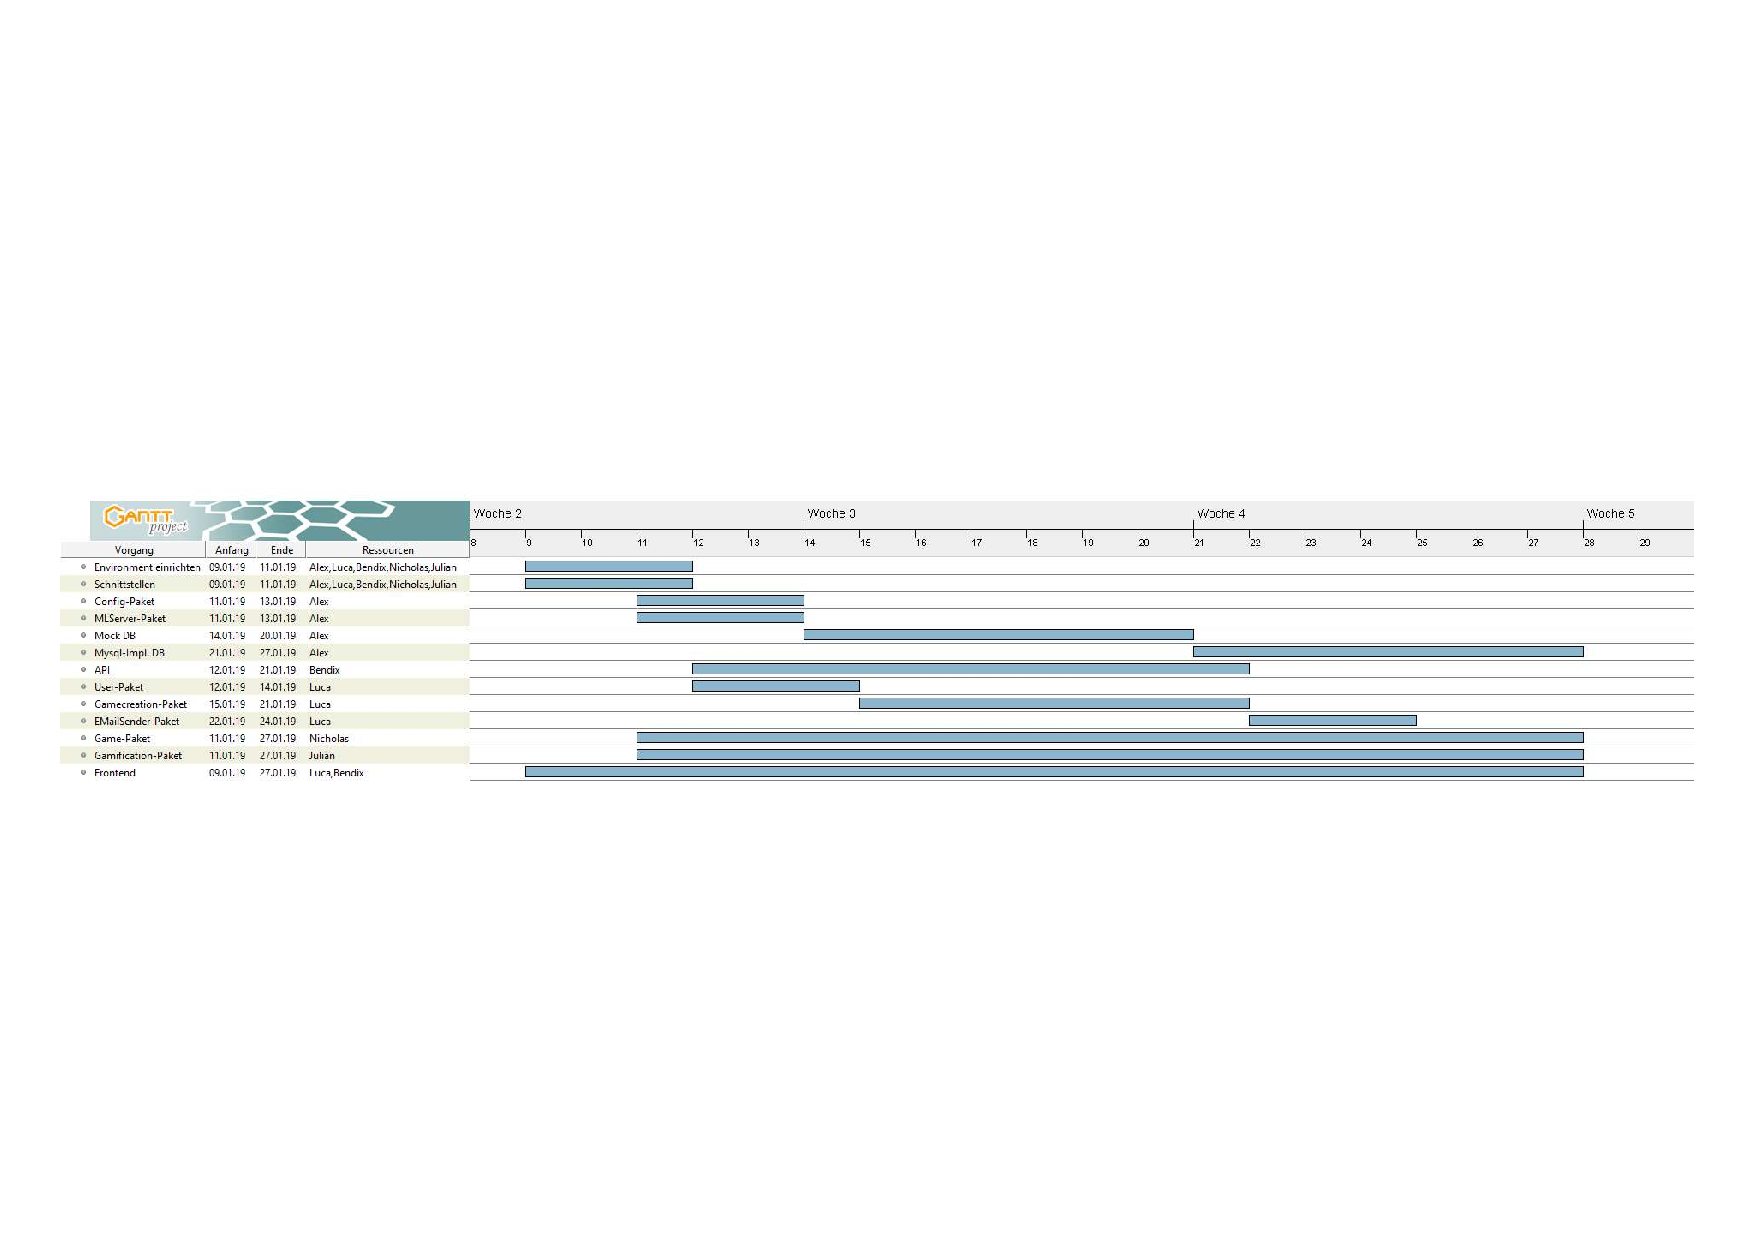
\includegraphics[width=\linewidth]{img/gantt.pdf}

\chapter{Unit-Tests}

	
\chapter{Anhang}





\end{document}